\begin{figure}
    \centering
    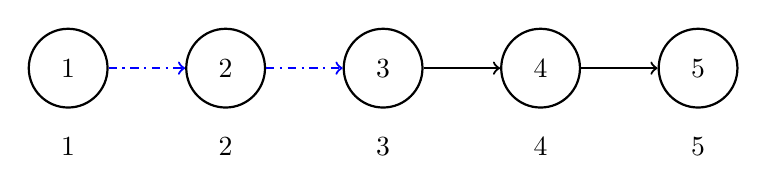
\begin{tikzpicture}[thick]
        \edef\pos{0}
        \foreach \x in {1, 2,..., 5}{
            \pgfmathparse{\pos+2}
            \xdef\pos{\pgfmathresult}
            \node[circle,draw, minimum size=1cm] (\x) at
                (\pos, 0) {$\x$};
            \node  at (\pos, -1) {$\x$};
        }
        % \foreach \x [evaluate=\x as \y using int(\x + 1)] in {1, 2,..., 4}{
        %     \ifthenelse{\x==2}{\draw[->, draw=red] (\x) -- (\y);}{\draw[->, draw=black] (\x) -- (\y);}
        % }
        \draw[->, color=blue, dashdotted] (1) -- (2);
        \draw[->, color=blue, dashdotted] (2) -- (3);
        \draw[->] (3) -- (4);
        \draw[->] (4) -- (5);
        % \draw[->] (1) edge (2) (2) edge (3) (3) edge (4) (4) edge (5)
    \end{tikzpicture}
    \caption[Certificados atualizados]{Após a mudança de trajetória do elemento 2,
            que se encontra em \sorted[2], \cert[1] e \cert[2]
            foram atualizados.}
    \label{fig:lista:after}
\end{figure}